\section{Background}
\label{sec:background}

\begin{figure*}[tb]
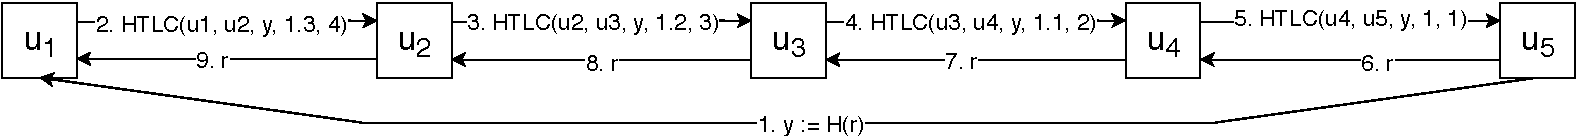
\includegraphics[width=\textwidth]{htlc-figure}
	\caption{An HTLC-based payment in the LN. The node $u_1$ pays $u_5$ using $u_2$, $u_3$ and $u_4$ as intermediaries. 
	Here we assume that each node charges a fee of $0.1$ and time is measured in days.\label{fig:htlc}}
\end{figure*}

The Lightning Network (LN) has emerged as the alternative to the scalability issue of Bitcoin  with the highest adoption in practice~\cite{Cuen2019}.
%LN has experienced rapid growth since its launch in early 2018~, 
As of February~2020, LN facilitates the off-chain exchange of nearly $900$~BTC.
The principles of the LN can be used to improve the scalability of other cryptocurrencies. 
For instance, similar networks operate with Litecoin~\cite{1MLLitecoin} and Ethereum~\cite{RaidenWebsite}. 
In this section, we introduce the basic notions of the LN and refer the reader 
to~\cite{Gudgeon2019} for further reading.
% TowardsBitcoinPaymentNetworks, BitcoinMagazineUnderstandingLightning, 

\subsubsection*{LN nodes} A node in the LN is governed by a pair of signing and verification keys from 
the ECDSA signature scheme, 
and identified by the hashed value of the verification key.  
Additionally, the owner can assign a handcrafted identifier (alias) to their node.
Operations from a node are authorized with a digital signature 
created with the corresponding signing key.
Thus, whoever holds the signing key is the owner of a node.
One user can potentially own several nodes.

%\vspace{-0.2cm}
\subsubsection*{LN channels} A LN channel (i.e.,~an edge) is jointly controlled by the two counterparties and its capacity is determined by the amount of coins 
deposited when created.
While the total capacity of the channel stays constant during its lifetime,
the balance of each counterparty varies according to two operations:
(i) single channel updates, where the two users agree on an updated balance; and 
(ii) multi-hop transactions, where the balance 
of several channels forming a path are simultaneously updated. 

%\vspace{-0.2cm}
\subsubsection*{LN transactions} A multi-hop transaction (or simply a transaction hereby) leverages a 
path of channels between a sender and a receiver (who might not share a channel between them).
A transaction must ensure the atomicity of the transfer: 
either all balances along the path are updated or none of them are.
For that, the LN relies on Hash Time-Lock Contracts (HTLCs), 
 excerpts from the  Bitcoin's scripting language that 
permit a node ($u_1$) to lock $x$~coins in a channel between two nodes ($u_1$ and $u_2$) 
and release them according to the encoded conditions.
The terms for the HTLC($u_1, u_2, y, x, t$) are defined with a hash value $y := H(r)$, 
where $r$ is chosen uniformly at random, 
an amount $x$ of coins, and a timeout $t$, as follows: 
(i) If $u_2$ reveals a value $r$ such that $H(r) = y$ before $t$ expires, $u_1$ pays $x$  to $u_2$; 
(ii) if $t$ expires, $u_1$ receives $x$  back.

LN relies on HTLCs to enable multi-hop transactions.  
All HTLCs along the path use the same hash value $y=H(r)$ aiming to achieve atomicity expecting that 
none of the intermediate balances can be updated before the receiver reveals $r$, and all of them can be updated after that.
An illustrative example of an HTLC-based transaction is depicted in~\cref{fig:htlc}.
Here, the user $u_1$ transfers $1$ bitcoin to $u_5$ using $u_2$, $u_3$ and $u_4$ as intermediaries. 
For that, $u_5$ locally chooses a value $r$ 
uniformly at random, computes the cryptographic challenge for the HTLC as $y := H(r)$, 
and sends $y$ to the sender (step 1).
The message encoding $y$ is called an \textit{invoice}.
Then, the payment starts with a commit phase (steps 2-5) where every pair of nodes, 
starting from the sender, establishes an HTLC using $y$.
After the commit phase is finished, the transaction enters the release phase.
Here, the receiver reveals $r$ to $u_4$ to fulfill the contract (step 6), 
triggering thereby the release phase where every pair of nodes fulfills their 
contract from the receiver to the sender (steps 6-9).

It is important to note two aspects here.
First, every intermediary user charges a fee for the forwarding service provided. 
For instance, $u_2$ receives $1.3$~coins but only forwards $1.2$~coins, getting a fee of $0.1$~coins. 
Second, the time parameter of the contracts throughout the path is decreasing to ensure that no user loses coins. 
For instance, the HTLC between $u_1$ and $u_2$ sets a timeout of four days 
whereas the timeout in the HTLC between $u_2$ and $u_3$ is only three days.
This facilitates that 
$u_2$ has enough time to settle the contract with $u_1$ after receiving $r$ from $u_3$.
%\todo[inline]{Mention that this introduces a DoS risk?}
% There is an inherent trade-off: channels with short timelocks open the risk of not being able to dispute a fraudulent transaction in case of blockchain congestion, and long timelocks open up a DoS vector, where an attacker can route many unsettled payments through a channel and effectively block it until the timelock expires.

%\todo[inline]{Preventing and onion routing paragraphs could be deleted}
%\paragraph{Preventing cheating}
%A critical problem for off-chain protocols is invalidating an old state.
%In a channel between Alice and Bob, after Alice has sent some \coins to Bob, she may try to close the channel on-chain, effectively double-spending.
%To prevent this, in every LN transactions the parties exchange secrets which would allow them to take all money from the channel should the other party publish an old state.
%
%\paragraph{Onion routing}
%A channel can keep track of multiple unsettled HTLCs.
%In a chain of channels "Alice - Bob - Charlie - Dave", Alice can be paying Dave, and at the same time Bob can be paying Dave.
%For each payment being forwarded, a node only knows the immediate previous and next hops, but neither the initial sender nor the final recipient.

\subsubsection*{LN implementations} 
The development of the LN, which was originally introduced in~\cite{Poon2016}, is guided by a set of request for comments (RFC) documents called "Basics of Lightning Technology" or BOLTs~\cite{BOLT}, 
which are then followed by several implementation teams.
The three most advanced implementations available today are LND~\cite{LND}, 
c-lightning~\cite{clightning}, and Eclair~\cite{Eclair}.
Additionally, there exist implementations at earlier stages of development:
Electrum~\cite{ElectrumWebsite, ElectrumLightningAnnounce}, lit~\cite{lit}, lpd~\cite{lpd}, ptarmigan~\cite{ptarmigan}, and rust-lightning~\cite{rustlightning}.
Our analysis is concerned with the definition of the LN as described in the BOLTs and thus the results 
apply equally to every implementation. 
